
% ----------------------------------------------------------------------------------------------------------------
% This .tex file (and associated .cls V3.2SP) *DOES NOT* produce:
%       1) The Permission Statement
%       2) The Conference (location) Info information
%       3) The Copyright Line with ACM data
%       4) Page numbering
% ---------------------------------------------------------------------------------------------------------------

%% A bit of setup for convenient switching between draft and production modes
\def\draft{1}
%% And the commands themselves
\newcommand{\ifdraft}[0]{\ifnum\draft=1}
\RequirePackage[final]{graphicx}

\ifdraft
\documentclass[draft,pdftex,letterpaper]{acm_proc_article-sp}
\newcommand{\PAGENUMBERS}{yes}       % "yes" or "no"
\else
\documentclass[pdftex,letterpaper]{acm_proc_article-sp}
\newcommand{\PAGENUMBERS}{no}       % "yes" or "no"
\fi


\usepackage{balance}  % to better equalize the last page
\usepackage{times}    % comment if you want LaTeX's default font
\usepackage{url}      % llt: nicely formatted URLs
\usepackage{tabularx}
\usepackage{float}
%\usepackage{color}
\usepackage{url}
\usepackage{algpseudocode}
\usepackage{algorithm}
\usepackage{verbatim}
\usepackage{mathtools}
\usepackage{caption}
\usepackage{subcaption}
%\usepackage{amsmath}
\let\proof\relax
\let\endproof\relax
\usepackage{amsthm}
\usepackage{thmtools}
\usepackage{xspace}
\usepackage{multirow}


%%%
%%%  Comments
%%%

\usepackage[usenames,dvipsnames]{color}

\ifdraft
\newcommand{\note}[2]{
    \textbf{\textcolor{#1}{#2}}\xspace
}
\else\newcommand{\note}[2]{\unskip}
\fi


%\newtheorem{lemma}{Lemma}[section]
%\theoremstyle{definition}
%\newtheorem{definition}{Definition}[section]
%\newtheorem{example}{Example}[section]

\declaretheorem[numberwithin=section]{definition}

\newcommand{\ie}{{\em i.e.}\xspace}
\newcommand{\eg}{{\em e.g.}\xspace}
\newcommand{\cf}{{\em c.f.}\xspace}
\newcommand{\ea}{{\em et al.}\xspace}
\newcommand{\aka}{{\em a.k.a.}\xspace}

\providecommand{\e}[1]{\ensuremath{\times 10^{#1}}}
\newenvironment{packed_item}{
\begin{itemize}
   \setlength{\itemsep}{1pt}
   \setlength{\parskip}{0pt}
   \setlength{\parsep}{0pt}
}
{\end{itemize}}

\newcommand\xqed[1]{%
  \leavevmode\unskip\penalty9999 \hbox{}\nobreak\hfill
  \quad\hbox{#1}}
\newcommand\marker{\xqed{$\square$}}

\newenvironment{packed_enum}{
\begin{enumerate}
   \setlength{\itemsep}{1pt}
   \setlength{\parskip}{0pt}
   \setlength{\parsep}{0pt}
}
{\end{enumerate}}

\renewcommand{\algorithmicrequire}{\textbf{Input:}}
\renewcommand{\algorithmicensure}{\textbf{Output:}}

\newdef{example}{\textit{Example}}

\begin{document}

\title{Benchmark Big Data Systems on Complex Analytic Queries}

% \numberofauthors{1}
% \author{
% \alignauthor
%  author1$^\dag$, author2$^{\dag,\S}$, author3$^\dag$\\
%        \affaddr{$^\dag$Computer Science and Engineering Department, University of Washington}\\
%        \affaddr{Seattle, Washington, USA}\\
%        \affaddr{$^\S$PETROBRAS S.A., Rio de Janeiro, RJ, Brazil}\\
%        \email{\{email1, email2, email3 \}@cs.washington.edu}
% }

\thispagestyle{empty}
\setcounter{page}{0}
\newpage


\maketitle

\begin{abstract}

In recent years, considerable number of big data systems emerged for
 large-scale data analyis following MapReduce. 
Most of the systems can handle the big volume of data if the analytic query 
itself is not complex.
In this paper, we would like to study how these systems perform against complex
queries. We consider the query is complex if the query has the following 
properties: 1) the query is iterative and cannot be done in a single round
of communication. 2) the query contains aggregates or UDFs which are widely
used for data analytics. 3) the query processes significant amount of data.
We proposed a benchmark consisting of a collection of such queries and
evaluated these queries on state-of-art representive big data systems in
its catagory. We think this emprical evaluation and analysis could be 
beneficial to the development of next generation big data systems.

\end{abstract}

%\category{H.2.4}{Database Management}{Systems}

%\terms{Management, Performance}

\begin{sloppypar}

\section{Introduction}

Following MapReduce, many big data analytics systems emerges in recent years, 
including Spark-SparkSQL \cite{XinRZFSS13SIGMOD, ZahariaCDDMMFSS12NSDI}, 
GraphLab \cite{GonzalezLGBG12OSDI}, Myria~\cite{HalperinACCKMORWWXBHS14SIGMOD} 
and others \cite{AbouzeidBARS09PVLDB,ThusooSJSCZALM10ICDE}. One similarity 
among these systems is that they all deploy in shared-nothing cluster and can 
scale well for relatively simple queries over large data due to massive 
parallelism. 

In this paper, we ask a vital question, how do these system perform if the
query is ``complex''. We characterize the query as complex if the query has 
the following properties.

\begin{enumerate}

\item \textbf{Iterative}. This means that the query requires some
iterative computation. Example can be like PageRank and graph reachability. 

\item \textbf{Aggregation and Filtering}. Aggregation means the final
result of the query is aggregated and contains possibly much less data
than input. This can be think of aggregation in SQL or \texttt{reduce} on data
by applying combining function. Data filtering means the input data needs to be
filtered by certain predicate of conditions. Both aggregation and filtering is 
not abnormal in data curating or ETL process.

\item \textbf{Multiple data sources}. This requires the input data of the 
query is from more than one data source or tables. This requirement is not
rare in practice and will require the system to handle data communication
properly since in many cases the system need to send data between servers.

\end{enumerate}

We choose this criteria from two different aspects of considerations. On one
 hand, these properties are not abnormal in analytic processes.
  For example, to 
get value from data, many algorithms like PageRank, K-Means require iterative
query. Also data analysts usually will spend a large portion of time to do ETL
or data curating, which requires the ability of aggregation and filtering. And 
in real world applications, data can usually comes from different data 
sources or tables and need to be combined together. On the other hand, these
properties requires clever system design and implementation to be efficiently
computed. And simple parallelization may not need to satisfactory 
performance. For example, pipelining hadoop jobs to execute iterative 
queries will suffer from Hadoop's huge cost of serialization and 
deserialization and the cost of synchronization between jobs. From these two 
perspective, we pick these properties to make this benchmark practical yet 
could be helpful to design future big data systems. 

We chooses three queries, least common ancestor in a citation graph, k-core
computation and myMergerTree edge computation, which have the properties that
we defined, to test the performance of the three big data systems. Our
objective evaluation contains two measures, lines of code (LOC), which 
measures how easy to write code using the programming abstraction offered by
a system, and query runtime, which measures the efficiency of the system.

We test our benchmark in three state of art big data systems. Myria, a shared
nothing parallel relational database system, whose programming model is SQL 
with iteration. Spark, a data flow based distributed computation engine, whose
 programming model is MapReduce. GraphLab, a distributed graph processing and 
machine learning engine, whose computation model is vertex based message
passing and aggregation (mainly support Gather, Apply and Scatter operations).

Our empirical evaluation shows that Myria has the fewest lines of code in all
three queries and has the fastest runtime in two of three queries (with the 
exception of LCA, which is 1.38x of GraphLab's runtime). Spark is comparable 
with Myria in LOC but is slowest among the three systems among the two queries
on which all three system successfully completed. GraphLab shows very good 
effciency however needs the most lines of code among all systems.

We also discussed our experience of using the three system in Section \ref{sec:comp}.



\section{Methodology}
    
\subsection{Systems that we compare}

\subsection{Metrics}

\section{Benchmark Queries}
\label{sec:benchmark}

\subsection{Q1: LCA}
This query is to compute the least common ancestor (LCA) of two 
academic papers. An ancestor of paper $p$ is transitively defined as:

\begin{enumerate}
    \item Any paper that $p$ cites is an ancestor of $p$
    \item Any paper that $p$'s ancestor cites is an ancestor of $p$
\end{enumerate} 

Given two paper $p_1$ and $p_2$, if their sets of ancestors are 
$a(p_1)$ and $a(p_2)$, their common ancestors are 
$a(p_1) \cap a(p_2)$. We define the distance from a common ancestor
as $d(a_1, p_1, p_2) = max(dist(a_1, p_1), dist(a_1, p_2))$, where 
$dist(a_1, p_1)$ is the minimum number of citation hops from $a_1$ to 
$p_1$. Then we can define a total ordering among the common ancestors
of $p_1$ and $p_2$ as, if $a_i, a_j \in a(p_1) \cap a(p_2)$, 
$a_i \prec a_j$ if and only if.

\begin{enumerate}
    \item $d(a_i, p_1, p_2) < d(a_j, p_1, p_2)$.
    \item $d(a_i, p_1, p_2) = d(a_j, p_1, p_2)$ and the year when $a_i$
    published $year(a_i)$ is earlier than $a_j$'s $year(a_j)$.
    \item if $d(a_i, p_1, p_2) = d(a_j, p_1, p_2)$ and $year(a_i) = year(a_j)$, $a_i$'s paper id is a smaller number than $a_j$'s.
\end{enumerate}

\subsection{Q2: K-Core}

The query is to compute the $k$-core (or $k$-degenerate graph) 
of an undirected graph. It is firstly defined by Paul Erd\H{o}s 
and Hajnal as color number \cite{ErdosH66}. 
$k$-core is an important structural property
and has been studied extensively in network analytics 
\cite{Alvarez-HamelinDBV05NIPS, ChengKCO11ICDE}.

A $k$-core of a graph $G$ is a maximal induced subgraph of $G$ in which all
vertices have degree at least $k$ in the subgraph. 
Figure~\ref{fig:k-core_example} shows $1 \ldots 3$-cores of a graph. 

\begin{figure}[t]
    \centering
    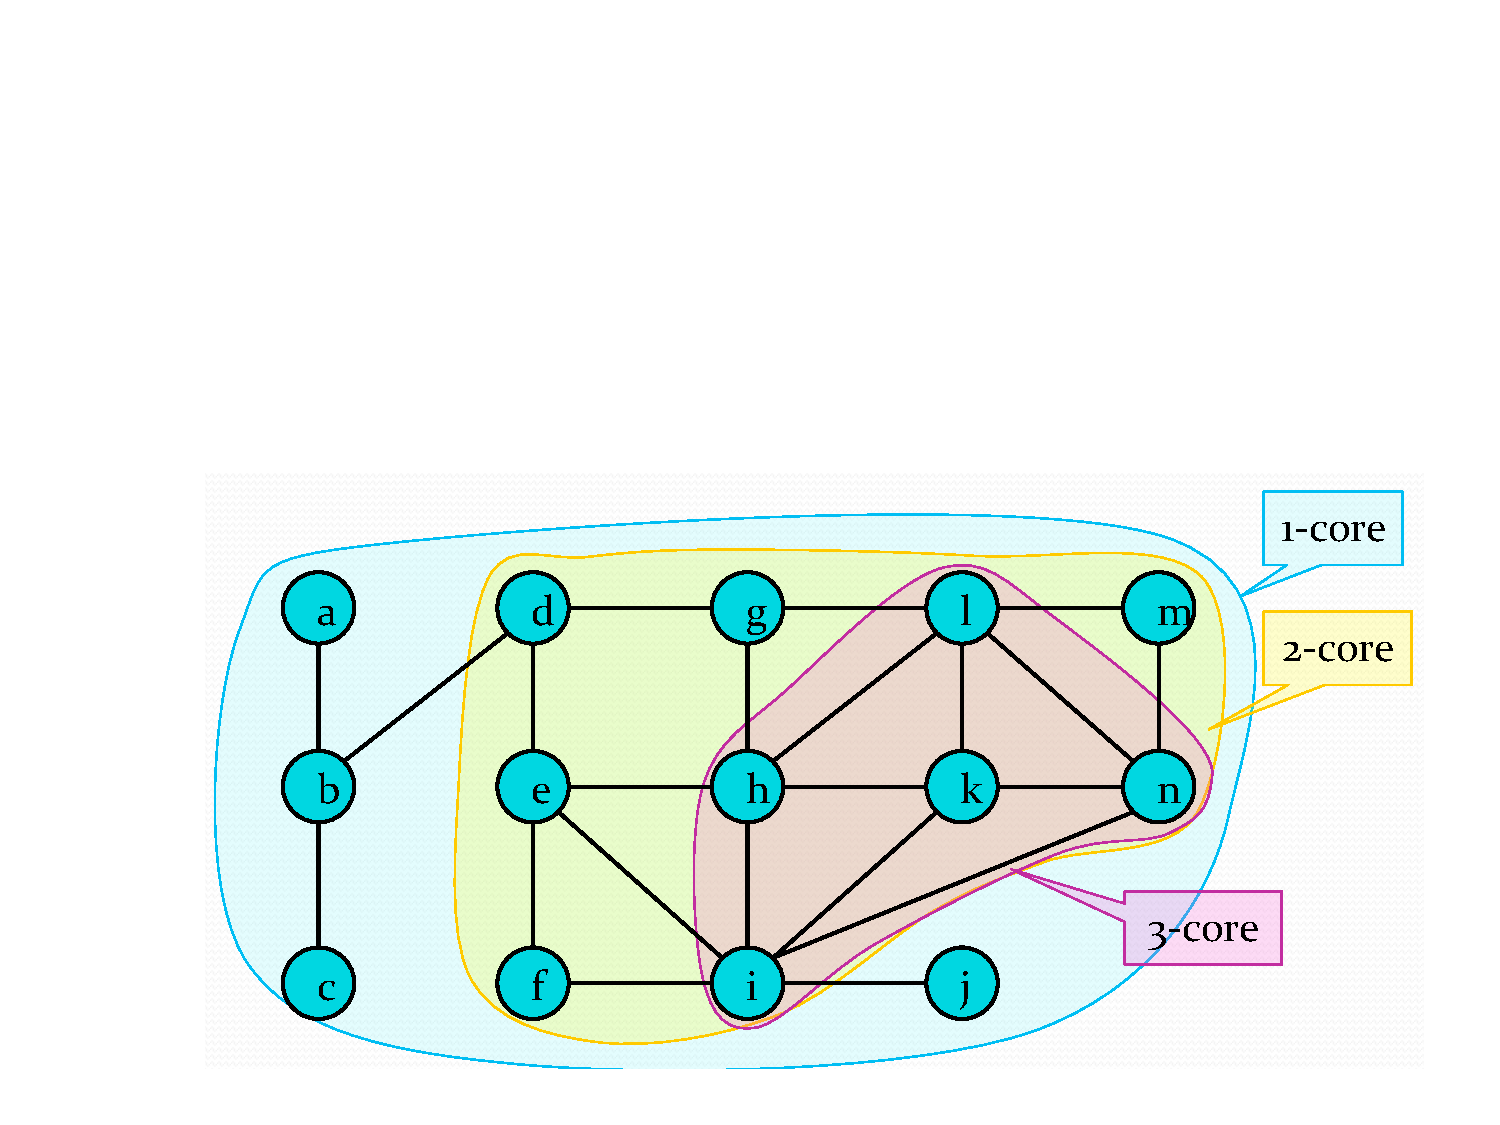
\includegraphics[width=0.9\linewidth]{images/kcore.pdf}
    \caption{Example of k-cores of a graph $G$}
    \label{fig:k-core_example}
\end{figure}

$k$-core has two interesting properties. First, as showed in 
Figure~\ref{fig:k-core_example}, $n$-core contains all the vertices 
in $n+1$-core. Second, there is a polynomial time ($O(m)$, $m$ is the 
number of edges of the graph) algorithm for 
core decomposition (compute all cores) \cite{BatageljM03CORR}.
Algorithm~\ref{alg:k-core} shows the algorithm of computing $k$-core.

\begin{algorithm}
\caption{Core Decomposition Algorithm}
\label{alg:k-core}
\begin{algorithmic}[1]
\Require k \Comment{k}
\Require G \Comment{Input Graph}
\While{true}
    \State $count \leftarrow 0$
    \ForAll{every vertex $v \in V(G)$}
        \If{$deg(v) < k$}
            \State remove $v$ from $V(G)$
            \State remove edges adjacent to $v$ from $E(G)$
            \State $count \leftarrow count+1$
        \EndIf
    \EndFor
    \If{$count = 0$}
        \State break.
    \EndIf
\EndWhile
\end{algorithmic}
\end{algorithm}

\subsection{Q3: Merger-Tree}

The merger tree query is from large-scale cosmological simulation in astronomy.
The astronomers want to track the evolution of galaxies from the Big Bang
to the present day, which spans over 14 billion years. The merger tree query 
compute the hierarchical assembly of galaxies by tracking the merging of 
small galaxies. In our evaluation, we assume that all the preprocessing has
been properly done and evaluate the 3rd computation step
 in \cite{LoebmanOCOAHBQG14SIGMOD}. The query will compute weighted edges
 (number of particles shared) between two galactic groups in two adjacent time
 stamp ($t$ and $t+1$). Also, this query only compute the edges related to a 
 set of particles that specified by the astronomers (Particles of interest).

 \begin{figure}[t]
 \begin{verbatim}
 particle(pid, grp_id, time) :- 
    poi(pid, grp_id, time), 
    halo(grp_id, time, totalParticles>256).
 
 edges(time, gid1, gid2, $count(*)) :-
    particle(pid, gid1, time), 
    particle(pid, gid2, time+1).
 
 treeEdges(1, gid1, gid2, count) :- 
    edges(time=1, gid1, gid2, count).

 treeEdges(time+1, gid2, gid3, count) :-
    treeEdges(time, gid1, gid2, count), 
    edges(time+1, gid2, gid3, count). 
 \end{verbatim}
 \caption{Merger Tree Query}
 \label{fig:merger-tree}
 \end{figure}

We show the datalog verison of this query in Figure~\ref{fig:merger-tree}. 
The query firstly uses halo table to filter out all the particles that are 
in the halo with total number of particles less or equal than $256$ 
(those are considered as insignificant halo by the astronomers). 
Then we computed all the edges by joining the particle particle table.
At last we compute all the tree edges, which only consider the edges that can
be traced ``back'' to current time. 

\section{Experimental Evaluation}

We report the experimental result of running three benchmark queries from 
Section~\ref{sec:benchmark}. We deployed the three systems in Amazon EC2 using 
the identical configuration, which uses 1 master node and 16 slave nodes.
Each node is a m3.large instance which has 2 vCPU, 7.5 GB RAM and 32GB SSD 
storage. We used the most up to date version of the 3 systems that we can get:
Myria (Daily built in Mar 10, 2015, commit: 90d85cd), Spark (1.2.1 release) and
GraphLab (Open sourced version in GitHub, commit: 18c2103).

\subsection{Q1}
\subsection{Q2}
\subsection{Q3}


\section{Conclusion}

We defined a benchmark which considering three important properties of modern
complex analytic queries. We evaluated three state of art big data systems 
which have different data model and programming abstraction over our benchmark
using the same instance setting in EC2. We discuss the pros and cons of these
systems and reported our experience on deploying and using these three systems.

\section{Acknowledgments}

We would like to thank Daniel Halperin for his MyriaL code on LCA and thank 
Maaz Ahmad and Antoine Kaufmann for their GraphLab code on LCA. We would like 
to thank Jennifer Ortiz and Laurel Orr for their help on myMergerTree query. 
We would like to thank Magdalena Balazinska for the helpful discussion on the
project.





\end{sloppypar}

\newpage

% \scriptsize
\bibliographystyle{abbrv}
\bibliography{report}

\end{document}
